\section{Time Complexity: Introduction}\label{sec:time_complexity_introduction}

\begin{frame}
	\frametitle{Time complexity}
	\framesubtitle{XKCD Algorithms: \url{https://xkcd.com/1667}}
	
	\begin{center}
		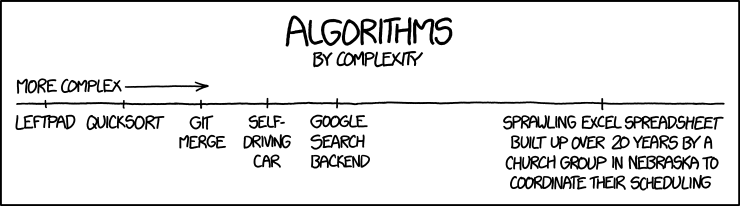
\includegraphics[width=0.9\textwidth]{figures/algorithms.png}
	\end{center}
\end{frame}


\begin{frame}
	\frametitle<-3>{What does it do?}
	\frametitle<4->{How fast does it do it?}

	\begin{overlayarea}{\textwidth}{\textheight}
		\lstinputlisting{code/for-loop.py}
		\pause
		\only<2-3>{
			\begin{questionblock}{What does it do?}
				What does the code compute?
			\end{questionblock}
			\only<3->{
				\begin{answerblock}{Sum of squares}
					\texttt{foo(n)} computes $\sum\limits_{i=0}^{n-1} i^2$
				\end{answerblock}
			}
		}
		\only<4->{
			\begin{questionblock}{How fast does it do it?}
				How fast is it?
			\end{questionblock}
			\only<5->{
				\begin{alertblock}{Harder to answer}
					1 second for $n=1000$.\\
					\only<6->{
						But what if $n$ changes?\\
						And what if we use another computer?
					}
				\end{alertblock}	
			}
		}
	\end{overlayarea}
\end{frame}

\begin{frame}
	\frametitle{Why do we ask this?}

	\begin{columns}
		\column{0.455\textwidth}
			\lstinputlisting{code/for-loop.py}
			\lstinputlisting{code/nested-for-loop.py}
		\column{0.455\textwidth}
		\pause
		\begin{questionblock}{Comparing implementations}
			How can we compare \texttt{foo} and \texttt{bar}?
		\end{questionblock}
		\pause
		\begin{answerblock}{Counting}
			By counting operations!
		\end{answerblock}
	\end{columns}
\end{frame}

\begin{frame}
	\frametitle{Counting operations}
	\begin{columns}
		\column{0.455\textwidth}
			\lstinputlisting{code/for-loop.py}
		\column{0.455\textwidth}
		\pause
		\begin{questionblock}{Counting operations}
			How many operations happen when we call \texttt{foo(n)}?
			\begin{enumerate}[A.]
				\item $2 + n$
				\item $2 + n + n$
				\item $3 + 2n + n-1$
				\item $4 + n + n + n + n-1$
			\end{enumerate}
		\end{questionblock}
	\end{columns}
	\pause
	\begin{answerblock}{Counting}
		It depends\dots
	\end{answerblock}
\end{frame}

\begin{frame}
	\frametitle{Getting rid of those nasty constants}

	\begin{itemize}
		\item Observation: We do not care if it's is $2+n$ or even $3+2n$.
		\item The important part is that it \textit{scales with the input}.
			\pause
		\item We call this the ``asymptotic run time complexity''.
	\end{itemize}
	\pause
	\lstinputlisting{code/for-loop.py}

	\begin{answerblock}{No more numbers}
		We say this code has $c_0 + c_1n$ operations, where:
		\begin{itemize}
			\item $c_0$ is initialisation of $s$ on line 2 and the return statement on line 5.
			\item $c_1$ is the \texttt{range} function on line 3 and the multiplication and addition on line 4.
		\end{itemize}
	\end{answerblock}
\end{frame}

\begin{frame}
	\frametitle{Getting rid of those nasty constants}

	\begin{overlayarea}{\textwidth}{\textheight}
			\lstinputlisting{code/nested-for-loop.py}
			\only<1>{
			\begin{questionblock}{So what about here?}
				How can we describe the number of operations here?	
			\end{questionblock}
		}
		\only<2>{
			\begin{answerblock}{Quadratic time}
				We say this code has $c_0 + c_1n + c_2 n^2$ operations, where:
				\begin{itemize}
					\item $c_0$ is initialisation of $s$ on line 2 and the return statement on line 6.
					\item $c_1$ is the \texttt{range} function on line 3.
					\item $c_2$ is the \texttt{range} function on line 4 and the multiplication and addition on line 5.
				\end{itemize}
			\end{answerblock}
		}
	\end{overlayarea}
\end{frame}

\begin{frame}
	\frametitle{So why does this matter?}
	\framesubtitle{Observing the differences}
\end{frame}

\begin{frame}
	\frametitle{Some numbers!}
	\framesubtitle{Check the code used to find these numbers on GitLab!}
	
	\begin{exampleblock}{Differences in run time}

		Different code snippets, all executed 1000 times.

		\hfill\\
		\begin{tabular}{c | c c c c c c c}
			\small
			Input size & constant & linear & quadratic & cubic & exponential & factorial\\
			\midrule
			\pause
			1 & $<$10 ms & $<$10 ms & $<$10 ms & $<$10 ms & $<$10 ms & $<$10 ms\\
			2 & $<$10 ms & $<$10 ms & $<$10 ms & $<$10 ms & $<$10 ms & $<$10 ms\\
			\pause
			5 & $<$10 ms & $<$10 ms & $<$10 ms & 36 ms & 40 ms & 210 ms\\
			\pause
			7 & $<$10 ms & $<$10 ms & $<$10 ms & 49 ms & 50 ms & \alert{$>$3000 ms} \\
			\pause
			10 & $<$10 ms & $<$10 ms & 23 ms & 78 ms & 84 ms & \alert{$>$3000 ms}\\
			\pause
			100 & $<$10 ms & $<$10 ms & 284 ms & \alert{$>$3000 ms} & \alert{$>$3000 ms} & \alert{$>$3000 ms} \\
			\pause
			1000 & $<$10 ms & 54 ms & \alert{$>$3000 ms} &\alert{$>$3000 ms} & \alert{$>$3000 ms} & \alert{$>$3000 ms} \\
			\pause
			10000 & $<$10 ms &  \alert{$>$3000 ms} &\alert{$>$3000 ms} &\alert{$>$3000 ms} & \alert{$>$3000 ms} & \alert{$>$3000 ms} \\
		\end{tabular}
	\end{exampleblock}	
\end{frame}

\begin{frame}
	\frametitle{Classifying these run times}
	\framesubtitle{XKCD: Formal Logic \url{https://xkcd.com/1033}}

	\begin{center}
	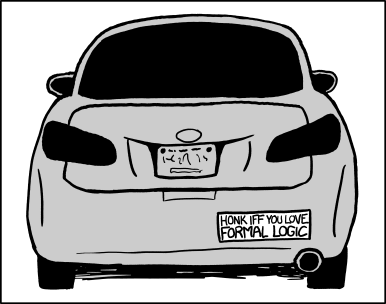
\includegraphics[width=0.6\textwidth]{figures/formal_logic.png}
	\end{center}
\end{frame}

\begin{frame}
	\frametitle{Big-Oh notation}

	\begin{itemize}
		\item We care about what we call: ``asymptotic run time complexity''.
		\item We denote this using big-Oh, e.g.\ $f(n) = 3n + 2$ is $O(n)$.
	\end{itemize}
	\pause
	\begin{questionblock}{A friend of mine told me...}
		Have you seen this notation before?
	\end{questionblock}
	\pause
	\begin{answerblock}{Something something, mathematics?}
	\begin{itemize}
		\item You (may?) have used big-Oh to a certain point before. E.g.\ as $n$ approaches $5$.
			\pause
		\item In computer science we only think about when $n$ approaches $\infty$.
	\end{itemize}
	\end{answerblock}
\end{frame}

\begin{frame}
	\frametitle{Formally}
	\begin{definition}[Big-Oh]
		A function $f(n)$ is $O(g(n))$ iff there is a positive real constant $c$ and a positive integer $n_0$ such that for
		all $n \geq n_0$ it holds that $f(n) \leq c g(n)$. In other words:\\
		$\exists c \in \mathbb{R}, \exists n_0 \in \mathbb{N} (c > 0 \wedge n_0 \geq 1 \wedge (\forall n \in \mathbb{N} (n
		\geq n_0 \to f(n) \leq cg(n))))$.
	\end{definition}
	\pause
	\begin{questionblock}{So...}
		Which of the following is/are true?
		\begin{enumerate}[A.]
			\item $n^2$ is $O(n^3)$
			\item $8n^2$ is $O(n^2)$
			\item $16n^2 + 5n + 2$ is $O(n^2)$
			\item $16n^2 + 5n \log n$ is $O(n^2)$
			\item $16n^2\log n$ is $O(n^2)$
		\end{enumerate}
	\end{questionblock}
\end{frame}

\begin{frame}
	\frametitle{Let's prove that shall we?}
	\framesubtitle{Well, I say ``we''...}

	\begin{questionblock}{}
		Prove that $f(n) = 16n^2 + 5n + 2$ is $O(n^2)$.
	\end{questionblock}
	\pause
	\begin{proof}
		To prove: $\exists c > 0, n_0 \geq 1$ such that $\forall n \geq n_0$ $16n^2 + 5n + 2 \leq cn^2$.\\
		\pause
		Take $n_0 = 1$, now for all $n \in \mathbb{N}$ with $n \geq n_0$:
		\begin{align*}
			16n^2 + 5n + 2 &\leq 16n^2 + 5n^2 + 2n^2 \\
										 &= 23n^2
		\end{align*}
		So take $c=23$.
	\end{proof}
\end{frame}

\begin{frame}
	\frametitle{Polynomial run time}
	
	\begin{definition}[Polynomial run time]
		A function has a polynomial run time $T(n)$ if $T(n)$ is $O(n^c)$ for some constant $c$.	
	\end{definition}
	\pause
	\begin{exampleblock}{This course}
		Most of the algorithms treated in this course have a polynomial run time.
	\end{exampleblock}	

	\pause
	\begin{alertblock}{Remember this}
		We will revisit the notion of polynomial run times in the very last lecture, where we study some problems that
		we believe to have no polynomial time solution!
	\end{alertblock}	
\end{frame}

\begin{frame}
	\frametitle{Some numbers! Revisited}
	\framesubtitle{Check the code used to find these numbers on GitLab!}
	
	\begin{exampleblock}{Differences in run time}

		We can now formalise our previous table a little bit:
		\pause

		\hfill\\
		\begin{tabular}{c | c c c c c c c}
			\small
			Input size & \alert{$O(1)$} & \alert{$O(n)$} & \alert{$O(n^2)$} & \alert{$O(n^3)$} & \alert{$O(2^n)$} & \alert{$O(n!)$} \\
			\midrule
			1 & $<$10 ms & $<$10 ms & $<$10 ms & $<$10 ms & $<$10 ms & $<$10 ms\\
			2 & $<$10 ms & $<$10 ms & $<$10 ms & $<$10 ms & $<$10 ms & $<$10 ms\\
			5 & $<$10 ms & $<$10 ms & $<$10 ms & 36 ms & 40 ms & 210 ms\\
			7 & $<$10 ms & $<$10 ms & $<$10 ms & 49 ms & 50 ms & $>$3000 ms \\
			10 & $<$10 ms & $<$10 ms & 23 ms & 78 ms & 84 ms & $>$3000 ms\\
			100 & $<$10 ms & $<$10 ms & 284 ms & $>$3000 ms & $>$3000 ms & $>$3000 ms \\
			1000 & $<$10 ms & 54 ms & $>$3000 ms &$>$3000 ms & $>$3000 ms & $>$3000 ms \\
			10000 & $<$10 ms &  $>$3000 ms &$>$3000 ms &$>$3000 ms & $>$3000 ms & $>$3000 ms \\
		\end{tabular}
		\pause
		\hfill\\
		Next lecture we will finish formalising this table.
	\end{exampleblock}	
\end{frame}

\begin{frame}
	\frametitle{Revisiting our code snippets}
	
	\lstinputlisting{code/for-loop.py}
	\begin{columns}
		\column{0.455\textwidth}
	\begin{questionblock}{So which is it?}
		Which of these describes the run time $T(n)$?
	\begin{enumerate}[A.]
		\item $T(n)$ is $O(1)$.
		\item $T(n)$ is $O(n)$. 
		\item $T(n)$ is $O(n^2)$. 
		\item $T(n)$ is $O(n^3)$. 
		\item I don't know.
	\end{enumerate}	
	\end{questionblock}
		\column{0.455\textwidth}
		\pause
		\begin{answerblock}{Multiple correct answers}
			B through D are correct.
		\end{answerblock}
		\pause
			\begin{block}{Tightest bound}
				We often request the tightest bound. Which in this case is $O(n)$.
			\end{block}	
	\end{columns}
\end{frame}

\begin{frame}
	\frametitle{Which case?}
	\lstinputlisting{code/for-loop-wc.py}
	\begin{columns}
		\column{0.755\textwidth}
	\begin{questionblock}{So which is it?}
		Which of these forms a tight bound on the run time $T(n)$?
	\begin{enumerate}[A.]
		\small
		\item $O(1)$. 
		\item $O(n)$. 
		\item $O(n^2)$. 
		\item I don't know.
	\end{enumerate}	
	\end{questionblock}
		\column{0.255\textwidth}
		\pause
		\begin{answerblock}{}
			Only B
		\end{answerblock}
		\pause
			\begin{block}{Worst Kaas}
				We talk about the \textit{worst-case}.
			\end{block}	
	\end{columns}
\end{frame}

\begin{frame}
	\frametitle{So...}
	\framesubtitle{There and back again}

	\begin{columns}
		\column{0.455\textwidth}
			\lstinputlisting{code/for-loop.py}
			\lstinputlisting{code/nested-for-loop.py}
		\column{0.455\textwidth}
		\begin{questionblock}{Comparing implementations}
			How can we compare \texttt{foo} and \texttt{bar}?
		\end{questionblock}
		\begin{answerblock}{Counting}
			\st{By counting operations!}\\
			\pause
			By comparing their asymptotic run time complexity!
		\end{answerblock}
		\begin{problemblock}{Issues?}
			What are the limitations?
		\end{problemblock}
	\end{columns}
\end{frame}


